\documentclass{article}

%% PAQUETES

% Paquetes generales
\usepackage[margin=2cm, paperwidth=210mm, paperheight=297mm]{geometry}
\usepackage[spanish]{babel}
\usepackage[utf8]{inputenc}
\usepackage{gensymb}

% Paquetes para estilos
\usepackage{textcomp}
\usepackage{setspace}
\usepackage{colortbl}
\usepackage{color}
\usepackage{color}
\usepackage{upquote}
\usepackage{xcolor}
\usepackage{listings}
\usepackage{caption}
\usepackage[T1]{fontenc}
\usepackage[scaled]{beramono}

% Paquetes extras
\usepackage{amssymb}
\usepackage{float}
\usepackage{graphicx}
\usepackage{array}
\usepackage{multirow}
\usepackage{amsmath}

%% Fin PAQUETES


% Definición de preferencias para la impresión de código fuente.
%% Colores
\definecolor{gray99}{gray}{.99}
\definecolor{gray95}{gray}{.95}
\definecolor{gray75}{gray}{.75}
\definecolor{gray50}{gray}{.50}
\definecolor{keywords_blue}{rgb}{0.13,0.13,1}
\definecolor{comments_green}{rgb}{0,0.5,0}
\definecolor{strings_red}{rgb}{0.9,0,0}

%% Caja de código
\DeclareCaptionFont{white}{\color{white}}
\DeclareCaptionFont{style_labelfont}{\color{black}\textbf}
\DeclareCaptionFont{style_textfont}{\it\color{black}}
\DeclareCaptionFormat{listing}{\colorbox{gray95}{\parbox{16.78cm}{#1#2#3}}}
\captionsetup[lstlisting]{format=listing,labelfont=style_labelfont,textfont=style_textfont}

\lstset{
	aboveskip = {1.5\baselineskip},
	backgroundcolor = \color{gray99},
	basicstyle = \ttfamily\footnotesize,
	breakatwhitespace = true,   
	breaklines = true,
	captionpos = t,
	columns = fixed,
	commentstyle = \color{comments_green},
	escapeinside = {\%*}{*)}, 
	extendedchars = true,
	frame = lines,
	keywordstyle = \color{keywords_blue}\bfseries,
	language = Octave,                       
	numbers = left,
	numbersep = 5pt,
	numberstyle = \tiny\ttfamily\color{gray50},
	prebreak = \raisebox{0ex}[0ex][0ex]{\ensuremath{\hookleftarrow}},
	rulecolor = \color{gray75},
	showspaces = false,
	showstringspaces = false, 
	showtabs = false,
	stepnumber = 1,
	stringstyle = \color{strings_red},                                    
	tabsize = 2,
	title = \null, % Default value: title=\lstname
	upquote = true,                  
}

%% FIGURAS
\captionsetup[figure]{labelfont=bf,textfont=it}
%% TABLAS
\captionsetup[table]{labelfont=bf,textfont=it}

% COMANDOS

%% Titulo de las cajas de código
\renewcommand{\lstlistingname}{Código}
%% Titulo de las figuras
\renewcommand{\figurename}{Figura}
\addto\captionsspanish{\renewcommand{\figurename}{Figura}}
%% Titulo de las tablas
\renewcommand{\tablename}{Tabla}
\addto\captionsspanish{\renewcommand{\tablename}{Tabla}}
%% Referencia a los códigos
\newcommand{\refcode}[1]{\textit{Código \ref{#1}}}
%% Referencia a las imagenes
\newcommand{\refimage}[1]{\textit{Imagen \ref{#1}}}



\begin{document}


% OBJETIVOS
\section{Objetivos}

	El objetivo del trabajo práctico es la familiarización con las propiedades, aplicaciones y utilización del osciloscopio como instrumento de visualización y medición de formas de onda. Además, se pretende el entendimiento del funcionamiento del osciloscopio y la adquisición de habilidades en el uso de los controles principales del panel frontal del mismo. Por último, se espera obtener una especial destreza en la realización de mediciones elementales.
\bigskip\bigskip




% INTRODUCCIÓN
\section{Introducción}

	El \textit{osciloscopio}, antiguamente conocido como \textit{oscilógrafo}, es un tipo de instrumento de medición electrónico que permite la representación gráfica de señales eléctricas que pueden variar en el tiempo. Presenta los valores de las señales eléctricas en forma de coordenadas en una pantalla, en la que normalmente el eje \textit{X} (horizontal) representa tiempos y el eje \textit{Y} (vertical) representa tensiones. La imagen así obtenida se denomina \textit{oscilograma}. 
	\par
	Las señales a menudo son periódicas, por lo que se repiten constantemente, de manera que, múltiples muestras de una señal que es en realidad variable en el tiempo se muestra como una imagen estable. Muchos osciloscopios (osciloscopios de almacenamiento) son también capaces de capturar formas de onda que no se repiten durante un tiempo determinado, mostrando en pantalla una forma estable del segmento capturado.
	\par
	Los osciloscopios se utilizan comúnmente para observar la forma de onda exacta correspondiente a una señal eléctrica. Estos son generalmente calibrados de manera tal que la tensión y el tiempo puedan ser percibidos de la mejor manera posible por el ojo humano. Esto permite la medición de, por ejemplo, la tensión pico a pico de una forma de onda, la frecuencia de señales periódicas, el tiempo entre pulsos, el tiempo que le toma a una señal para alcanzar su máxima amplitud (tiempo de crecimiento o subida), y el tiempo relativo entre varias señales relacionadas.
\bigskip\bigskip




% MATERIALES UTILIZADOS
\section{Materiales utilizados}

	Se detallan a continuación (\textit{Tabla 1}) la lista de materiales y dispositivos utilizados durante el desarrollo de la práctica, acompañados por sus respectivas características y especificaciones principales. Para más información sobre el instrumental puede dirijirse a la sección \textit{Apéndice B}, ubicada al final del presente informe, donde se adjuntan las hojas de datos de todos estos.
\bigskip\bigskip


% Tabla 1
\begin{table}[!hbt]
	\begin{center}
	\begin{tabular}{|>{\centering\arraybackslash}m{5cm}|>{\arraybackslash}m{6cm}|}
		\hline
		\rowcolor[gray]{0.9}\textbf{Material/Instrumento} & \textbf{Especificaciones} \\
		\hline
		\centering Resistencias & 47$\Omega\pm5\%$ tolerancia (1 unidad) \\
		\hline
		\centering Capacitores & 22$\mu$F, 50V (1 unidad) \\
		\hline
		Generador de funciones & Modelo: 8140\\
		\hline
		Osciloscipio & \vbox{\hbox{\strut Marca: GOOD-WILL }
						   \hbox{\strut Modelo: 653G }}\\
		\hline
		Contador & \vbox{\hbox{\strut Marca: GOOD-WILL }
						   \hbox{\strut Modelo: guc-2020 }}\\
		\hline
		Fuente regulada & \vbox{\hbox{\strut Marca: Hewlett-Packard }
						   \hbox{\strut Modelo: 721A }}\\
		\hline
		Multímetro digital & UNI-T Mod. UT30F \\
		\hline
		Cables & Banana-Cocodrilo\newline Cocodrilo-Cocodrilo\newline BNC-BNC\newline Banana-BNC \\
		\hline
	\end{tabular}
	\caption{Listado de materiales e instrumental utilizado.}
	\end{center}
\end{table}
\bigskip\bigskip
\newpage




% DIAGRAMA EN BLOQUES DEL OSCILOSCOPIO
\section{Diagrama en bloques del osciloscopio}

	Nos centraremos primeramente en comprender el funcionamiento de un osciloscopio, de manera de conocer los procesos internos llevados a cabo por el aparato. Esto nos ayudará más adelante en el entendimiento del funcionamiento de los controles que posee este instrumento. Cabe aclarar que solamente nos referiremos al funcionamiento básico y general de los osciloscopios analógicos.
	\par
	En la \textit{Figura 1} se muestra un diagrama en bloques en el que se situan los controles principales de un osciloscopio. A lo largo de los próximos tres apartados analizaremos cada parte de dicho diagrama, haciendo énfasis en cómo es que se va modificando la señal desde que ingresa hasta que llega a la pantalla.
\bigskip\bigskip


% Figura 1
\begin{figure}[h]
	\centering
	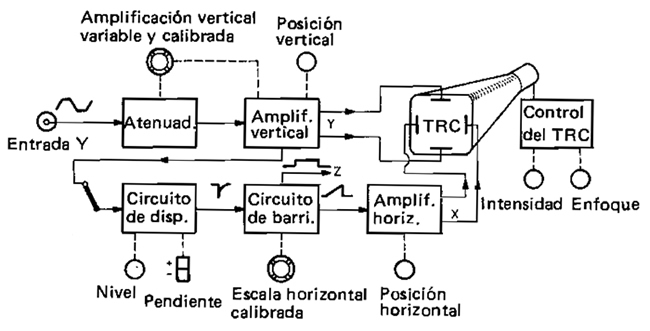
\includegraphics[width=0.85\textwidth]{images/01-diagrama-bloques-osc.jpg}
	\medskip
	\caption{Diagrama en bloques en el que se muestran los controles\\ principales de un osciloscopio.}
\end{figure}
\bigskip



% DIAGRAMA EN BLOQUES DEL OSCILOSCOPIO - Sistema vertical simplificado
\subsection{Sistema vertical}
	
	Cuando se conecta la sonda del osciloscopio (ó mas técnicamente \textit{probe}) a un circuito, la señal atraviesa a ésta ingresando por la \textit{Entrada Y} y se dirige directamente a la sección vertical. Allí se situa en el \textit{Atenuador}, donde es atenuada en la medida en que el usuario disponga. Dependiendo de donde situemos el mando del amplificador vertical atenuaremos la señal o la amplificaremos. Luego la señal pasa al siguiente bloque, \textit{Amplificación vertical}, en donde es vuelta a amplificar. La razón por la cual se atenúa para más tarde amplificarla es a causa de lo costoso que es implementar un amplificador variable.
	\par
	A la salida del bloque de \textit{Amplificación vertical} ya se dispone de la suficiente señal para atacar las placas de deflexión verticales del tubo de rayos catódico, que naturalmente están en posición horizontal. Estas son las encargadas de desviar el haz de electrones, que surge del cátodo e impacta en la capa fluorescente del interior de la pantalla en sentido vertical: hacia arriba si la tensión es positiva con respecto al punto de referencia (\textit{GND}) ó hacia abajo si es negativa.
	\bigskip
	


% DIAGRAMA EN BLOQUES DEL OSCILOSCOPIO - Sistema horizontal simplificado
\subsection{Sistema horizontal}
	
	El sistema horizontal es el encargado de controlar que porción de la señal se visualizará en la pantalla del osciloscopio. La señal, al salir del bloque de \textit{Amplificación vertical}, además de dirigirse hacia las placas de deflexión verticales, se hace lugar hacia el \textit{Circuito de disparo}. Allí se inicia el barrido horizontal, siendo este bloque el encargado de mover el haz de electrones desde la parte izquierda de la pantalla hacia la parte derecha en un determinado tiempo. El trazado (recorrido de izquierda a derecha) se consigue aplicando la parte ascendente de un diente de sierra a las placas de deflexión horizontal las cuales se encuentran dispuestas verticalmente. Este puede ser regulable en tiempo actuando sobre el selector de base de tiempo. El trazado inverso, es decir, cuando el haz recorre el camino de derecha a izquierda, se realiza de forma mucho más rápida mediante la componente descendente del mismo diente de sierra.
	\bigskip\bigskip



% DIAGRAMA EN BLOQUES DEL OSCILOSCOPIO - Acople del sistema vertical con el sistema horizontal
\subsection{Acople del sistema vertical con el sistema horizontal}

	[ Colocar texto aquí ]
	\bigskip\bigskip




% CONTROLES DEL OSCILOSCOPIO
\section{Controles del osciloscopio}

	Pasaremos ahora a definir en forma resumida el funcionamiento de cada perilla del osciloscopio. 
\bigskip

\renewcommand{\labelenumi}{(\alph{enumi})}
\begin{enumerate}

	%% ITEM (a)
	\item \textbf{Controles del haz}\bigskip \\ 
		  \textit{Intensidad:} permite regular la intensidad del trazo en la retícula; \medskip \\ 
		  \textit{Foco:} controla el enfoque del trazo en la pantalla; \medskip \\
		  \textit{Iluminación:} permite regular la iluminación sobre la pantalla; \medskip \\
		  \textit{Rotación del trazo:} permite ajustar la posición horizontal del trazo, alineándolo angularmente con la cuadrícula que puede observarse sobre la reticula. \medskip \\

	%% ITEM (b)
	\item \textbf{Controles del canal vertical} \bigskip \\ 
		  \textit{Modo vertical:} permite elegir lo que se mostrará en el display: CH1 (canal 1), CH2 (canal 2), Dual (ambos canales a la vez) y Add (suma de las señales de ambos canales); \medskip \\
		  \textit{Chop:} modo en el cual, el osciloscopio traza una pequeña parte del Canal 1, luego otra pequeña parte del Canal 2, hasta completar un trazado completo y comenzar nuevamente. Se utiliza en señales de baja frecuencia, es decir, con la base de tiempo en posición de 1mS o superior; \medskip \\
		  \textit{CH2 Inv:} invierte la entrada del Canal 2; \medskip \\
		  \textit{Position:} permite mover verticalmente la forma de onda hasta el punto exacto que se desee; \medskip \\
		  \textit{VOLT/DIV:} conmutador de varias posiciones, cada una de las cuales, representa el factor de escala empleado por el sistema vertical; \medskip \\
		  \textit{AC-DC:} acoplamiento que bloquea mediante un capacitor la componente continua que posea la señal exterior; \medskip \\
		  \textit{GND:} desconecta la señal de entrada del sistema vertical y lo conecta a masa, permitiendo situar el punto de referencia en cualquier parte de la pantalla; \medskip \\
		  \textit{VAR:} La rotación de este control facilita un ajuste fino de la sensibilidad vertical. Esto permite que la forma de onda pueda ser ajustada a número exacto de divisiones, aún cuando las medidas verticales no sean las realmente indicadas en el control de sensibilidad VOLTS/DIV. Este control debe estar normalmente en la posición CAL, es decir, calibrado. \medskip \\

	%% ITEM (c)
	\item \textbf{Horizontal} \bigskip \\ 
		  \textit{A Time/div:} conmutador de varias posiciones, cada una de las cuales, representa el factor de escala (en segundos por división) empleado por el sistema horizontal; \medskip \\
		  \textit{SWP VAR:} permite ajustar en forma continua entre las distintas escalas; \medskip \\
		  \textit{Position:} permite mover horizontalmente la forma de
onda hasta el punto exacto que se desee; \medskip \\
		  \textit{B Time/div:} controla la cantidad de segundos por división de la base de retardo; \medskip \\
		  \textit{$\times$10 Mag:} permite amplificar o magnificar por 10 la escala de tiempo; \medskip \\
		  \textit{X-Y:} permite desconectar el sistema de barrido interno del osciloscopio, haciendo estas funciones uno de los canales verticales (generalmente el Canal 2). Esto nos da la posibilidad de visualizar curvas de respuesta ó las figuras de Lissajous. \medskip \\

	%% ITEM (d)
	\item \textbf{Disparo} \bigskip \\ 
		  \textit{Trigger source:} selector que establece con respecto a que señal de entrada se establecerán los disparos; \medskip \\
		  \textit{Coupling:} conmutador con el que es posible conseguir el disparo estable de la señal en diferentes situaciones (e.g. AC, DC, HF, LF, LINE); \medskip \\
		  \textit{Slope:} selector que establece si el disparo debe efectuarse cuando la pendiente de la señal es positiva o negativa; \medskip \\
		  \textit{Level:} permite, en el modo de disparo manual, ajustar el nivel de
señal a partir del cual, el sistema de barrido empieza a actuar. Este ajuste no es operativo en modo de disparo automático; \medskip \\
		  \textit{Level lock:} bloquea el control Level; \medskip \\
		  \textit{Normal/Auto/Single:} selector del modo de disparo. En el modo NORMAL la señal que se muestra correspondie siempre al último barrido. Si no se produce disparo, la señal se congela en pantalla. En el modo AUTO, aunque no se produzca la condición de disparo, el osciloscopio esperará un tiempo y hará un barrido. En el modo SINGLE ó SINGLE TRIGGER, el osciloscopio realizará un único barrido, congelando la información en pantalla. Este modo sirve para ver transitorios que ocurren una sola vez;   \medskip \\
		  \textit{Holdoff:} establece el período de tiempo durante el cual el osciloscopio espera antes de volver a armar el sistema de circuitos de disparo (trigger). Es decir, inhibe ciertos disparos para que no ocurra el solapamiento de la señal cuando se introducen formas de onda complejas a la entrada; \medskip \\
		  \textit{Horizontal Display(A; A int. B; B; B Trig B):} \textit{A} muestra la base de tiempo principal. \textit{A int B} muestra la base de tiempo principal intensificada. \textit{B} muestra la base de tiempo secundaria. \textit{Trig B} muestra la base de tiempo secundaria intensificada.  \medskip \\

\end{enumerate}



% INCERTEZAS EN EL OSCILOSCOPIO
\section{Incertezas en el osciloscopio}

	[ Colocar texto aquí ]
\bigskip\bigskip



% MEDICIONES CON EL OSCILOSCOPIO
\section{Mediciones con el osciloscopio}

	Primeramente, para lograr un punto luminoso centrado en la pantalla del osciloscopio que sea circular, se pondrán las perillas del selector de entrada de los canales \textit{CH1} y \textit{CH2} en la posición \textit{GND}. De esta manera, internamente se conectan las entradas a masa. Luego se debe seleccionar el botón \textit{X-Y}\footnote{Dependiendo del modelo de osciloscopio utilizado puede que, en vez de un botón, dicha opción se encuentre en la última posición de la derecha del selector de base de tiemo \textit{TIME/DIV}.} del sistema horizontal. Para centrar el punto se debe hacer uso de las perillas de posición del sistema vertical y horizontal.	Este primer procedimiento realizado es útil para fijar la referencia del cero de la medición. También nos es de utilidad para centrar las figuras de Lissajous.
	\par
	Trabajaremos ahora junto al generador de funciones, al cual configuraremos para obtener a su salida una señal sinusoidal de 2Vpp y 1kHz. La salida de este debe ser conectada directamente al canal \textit{CH1} del osciloscopio con un cable \textit{BNC-BNC}. Para lograr sincronizar la señal se deben poner los controles del instrumento en el estado que denominaremos \textit{Estado inicial}:
\medskip


\begin{itemize}
\itemsep=2pt \topsep=0pt \partopsep=0pt \parskip=0pt \parsep=0pt
	\item \textit{Trigger LEVEL} = 0V
	\item \textit{Trigger SLOPE} = + (positivo)
	\item \textit{Trigger MODE} = Auto
	\item \textit{VOLT/DIV} = 0,5V
	\item \textit{TIME/DIV} = 0,2mS
	\item \textit{Vertical Position} = 0V al centro
\end{itemize}
\medskip


	Habiendo establecido este estado inicial en el osciloscopio, se pasó a medir la amplitud pico máxima del generador de funciones. Para lograrlo se posicionó la perilla del selector de entrada del canal CH1 en AC. Además, se debió modificar la escala de tensión de dicho canal a 5V/div y se tuvo que variar la perilla de posición vertical de manera de conseguir una lectura más comoda de la cantidad de divisiones abarcadas por la señal. Hecho esto se obtuvo el siguiente valor de tensión:

\begin{equation*}
	V_p(m\acute{a}x) = 11V \pm 0,5V
\end{equation*}
\medskip
	
	Luego se midió el periodo mínimo que nos puede entregar el generador de funciones (o lo que es equivalente, la frecuencia máxima), obteniéndose

\begin{equation*}
	p_{min} = 0,1\mu S \pm 0,01\mu S
\end{equation*}
\medskip

\noindent Para hacerlo se debió modificar la base de tiempo a XXXX XX/div y se tuvo que variar la perilla de posición horizontal de manera de conseguir una lectura mas cómoda de la cantidad de divisiones abarcadas por un ciclo de la señal.
	\par
	Para la medición del offset máximo que nos puede entregar el generador de funciones se procedió volviendo al estado inicial, manteniendo la conexión del generador de funciones al osciloscopio. Luego se aumentó la perilla del offset del generador al máximo (positivo). En el osciloscopio se posicionó la perilla del selector de entrada del canal \textit{CH1} en \textit{GND} y variando el potenciometro de posición vertical se llevó la señal hacia la segunda división mas baja de la pantalla. Acto seguido, se posicionó la perilla del selector de entrada del \textit{CH1} en \textit{DC} notando el desplazamiento de la señal a divisiones por encima de lo que llega a mostrar el display. Para lograr ver a esta de la forma mas conveniente se modificó la escala de tensión a 2V/div. Hecho esto se observó que el offset máximo (positivo) del generador de funciones es

\begin{equation*}
	Offset_{m\acute{a}x}(gen) = \pm (10,8V \pm 0,2V)
\end{equation*}
\medskip


\noindent En esta última medición hemos incluido el valor máximo negativo del offset ya que la medición debe realizarse de la misma manera pero invirtiendo la posición de la señal cuando se ajusta la perilla del selector de entrada del canal \textit{CH1} en \textit{GND}; es decir, en vez de colocarla en la segunda división más baja debemos colocarla en la segunda división mas alta de la pantalla ya que al disminuir al máximo el offset y al posicionar la perilla del selector de entrada del \textit{CH1} en \textit{DC} dicha señal se desplazará hacia abajo.
	\par
	Ahora mediremos el offset máximo pero el correspondiente al que puede entregar internamente el osciloscopio. Para lograrlo, partiendo del estado inicial y desconectando el generador de funciones utilizado en párrafos anteriores, conectaremos la fuente regulada al osciloscopio mediante un cable \textit{Banana-BNC} teniendo en cuenta el detalle de colocar la tensión de salida del primero en 0V. Además colocaremos un voltímetro en paralelo a la fuente, de manera de poder saber que tensión está entregando realmente, ya que la indicación de la propia fuente no es confiable. En el osciloscopio posicionaremos la perilla del selector de entrada del canal \textit{CH1} en \textit{GND} y variaremos el potenciometro de posición vertical hasta que este llegue a su máximo, es decir, cuando ya no sea posible seguir girándola hacia la derecha. Luego volveremos a modificar la posición de la perilla del selector de entrada del canal \textit{CH1} colocándola en \textit{DC}. Como puede notarse, la señal ya no se verá en la pantalla. Nuestro trabajo será entonces buscar ver de nuevo dicha señal alineada a la división de 0V del display. Para esto comenzaremos a aumentar la tensión de la fuente regulada hasta lograr dicha alineación. Una vez conseguido esto leeremos el valor de tensión medido por el voltímetro, siendo este el offset máximo entregado por el osciloscopio. Para el modelo utilizado en este informe se ha observado que dicho offset máximo es 

\begin{equation*}
	Offset_{m\acute{a}x}(osc) = 8 Div \times Escala
\end{equation*}
\medskip


	Si desearamos ahora medir la sensibilidad especificada por el fabricante del osciloscopio, podremos hacerlo conectando el generador de funciones al instrumento y agregándole un voltímetro digital en paralelo. De esta manera, y dejando el \textit{Level} en un valor muy cercano a cero, se debería ir variando la amplitud del generador, en busca del momento en donde la imagen queda sincronizada. En ese instante debe leerse la medición del voltímetro. Para esta experiencia convendría utilizar el modo de disparo único del osciloscopio, además de regular el canal vertical en una escala de 50 mV/div o similar.
\bigskip



% MEDICIONES CON EL OSCILOSCOPIO - Modo X-Y y figuras de Lissajous
\subsection{Modo X-Y y figuras de Lissajous}

\bigskip



% MEDICIONES CON EL OSCILOSCOPIO - Modo normal y automático
\subsection{Modo normal y automático}

	

\bigskip\bigskip	




% CONCLUSIONES
\section{Conclusiones}

	[ Colocar texto aquí ]
	\bigskip\bigskip




% APÉNDICE A

\newpage
\vspace*{4cm}
\begin{center}
	\textbf{\Huge{Apéndice A}} \\
	\bigskip\bigskip
	\Large{\textit{``Hojas de datos de instrumentos de medición''}}
\end{center}

\end{document}
